\documentclass{article}

\usepackage{hyperref}
\usepackage[T1]{fontenc}
\usepackage{graphicx}
\usepackage{float}
\usepackage[utf8]{inputenc}


\title{%
Laboratorium 5\\
  \huge Aproksymacja}
\author{Mateusz Król}
\date{17/04/2024 r.}

\begin{document}
\maketitle


\section*{Zadanie 1.}
\textbf{Wykonaj aproksymację średniokwadratową punktową populacji
Stanów Zjednoczonych w przedziale $[1900;1980]$ wielomianami stopnia $m$ dla
$0 \leq m \leq 6$.}
\newpage
Wykres błędów względnych w zależności od liczby węzłów wielomianu 
interpolacyjnego:
\begin{figure}[H]
  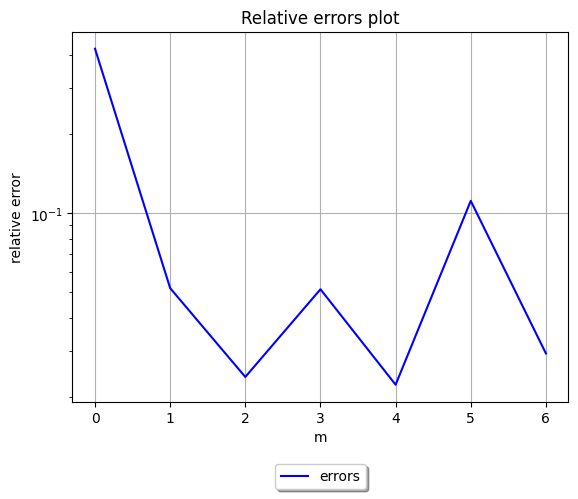
\includegraphics[width=\linewidth]{figures/errors.png}
\end{figure}
\newpage
Wykres wartości skorygowanego kryterium informacyjnego \textit{Akaike} 
($AIC_c$) w zależności od liczby węzłów wielomianu 
interpolacyjnego:
\begin{figure}[H]
  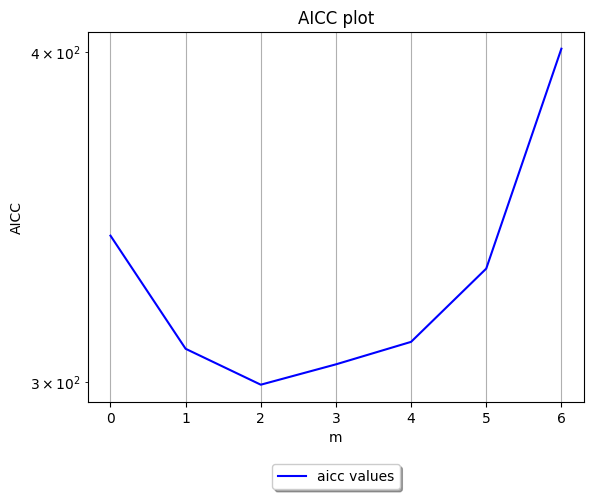
\includegraphics[width=\linewidth]{figures/aicc.png}
\end{figure}

\section*{Zadanie 2.}
\textbf{Wykonaj aproksymację średniokwadratową ciągłą funkcji}
$f(x) = \sqrt{x}$ \textbf{w przedziale} $[0;2]$ \textbf{wielomianem drugiego stopnia, używając wielomianów
Czebyszewa.}
\newpage
Wykres przedstawiający porównanie prawdziwych wartości funkcji 
$f(x) = \sqrt{x}$ oraz wartości aproksymowanych używająć wielomianów
\textit{Chebyshev}'a.
\begin{figure}[H]
  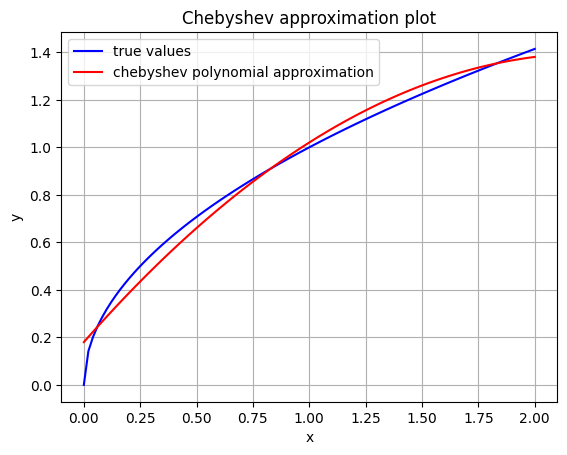
\includegraphics[width=\linewidth]{figures/chebyshev.png}
\end{figure}


\subsection*{Wnioski}
\null\quad W zadaniu 1, błąd względny był najmniejszy dla $m=2,4$, co
zgadza się z odpowiednio najmniejszą wartością $AIC_c$ dla $m=2$.


\end{document}